\documentclass[a4paper, 11pt]{article}
\usepackage[dvipsnames]{xcolor}
\usepackage{graphicx} % Required for inserting images
\usepackage{amsfonts}
\usepackage{amssymb}
\usepackage{amsmath}
\usepackage{tikz,lipsum,lmodern}
\usepackage[most]{tcolorbox}
\usepackage{pgfplots}
\usepackage{tabularx}
\usepackage{stmaryrd}
\usepackage{tikz} 
\usepackage{imakeidx}
\usepackage{blindtext}
\usepackage{hyperref}
\usepackage[rightcaption]{sidecap}
\usepackage{wrapfig}
\usepackage{cancel}
\usepackage{titlesec}
\usepackage{enumitem}
\usepackage{float}
\usepackage{markdown}

\titleformat{\chapter}[display]
  {\normalfont\Large\bfseries} % Stile del titolo
  {\chaptername\ \thechapter}{10pt}{\Large}

\titlespacing*{\chapter}{0pt}{-20pt}{20pt}


\hypersetup{
    colorlinks=true,
    linkcolor=black,
    filecolor=magenta,      
    urlcolor=blue,
    pdftitle={Relazione_Centro-Controllo-Droni},
    pdfpagemode=FullScreen,
}

\setlength{\parindent}{0pt}
\setlength{\parskip}{5pt}


\makeindex[columns=3, title=Alphabetical Index, intoc]
\hypersetup{
    colorlinks=true,
    linkcolor=blue!50!green,
    filecolor=magenta,      
    urlcolor=cyan,
    pdftitle={Overleaf Example},
    pdfpagemode=FullScreen,
    }

\newcommand\scalemath[2]{\scalebox{#1}{\mbox{\ensuremath{\displaystyle #2}}}}
\definecolor{bananamania}{rgb}{0.98, 0.91, 0.71}
\definecolor{amaranth}{rgb}{0.9, 0.17, 0.31}
\definecolor{amethyst}{rgb}{0.6, 0.4, 0.8}
\definecolor{darktangerine}{rgb}{1.0, 0.66, 0.07}
\definecolor{cerise}{rgb}{0.87, 0.19, 0.39}
\definecolor{babyblue}{rgb}{0.54, 0.81, 0.94}


\title{Relazione su \\
Controllo formazione droni}
\author{A. Bettoni (1998044),\\ A. Coppola (2003964),\\S. Di Cesare (1938649)}
\date{\today}

\begin{document}
\maketitle
\newpage
\tableofcontents
\newpage
\section{Descrizione Generale}
\paragraph*{Problema:}
Si vuole progettare un sistema di controllo di n droni che sorvegli una data area rettangolare.
Il sistema deve garantire che, con i droni forniti, ogni punto dell'area venga sorvegliato il più frequentemente possibile.

I droni partiranno dalla torre di controllo che si trova al centro dell'area da sorvegliare.
Ogni drone ha un'autonomia limitata (misurata in minuti in volo) e una velocità massima. 
La torre dovrà gestire gli spostamenti di ogni drone facendo in modo che tornino alla torre prima che la batteria sia del tutto esaurita. 
Quando i droni si trovano nella torre di controllo sono considerati in carica e il tempo di ricarica può variare da drone a drone.
\paragraph*{Idea di soluzione:}
Abbiamo scelto di modellare il problema con un sistema che agisce sulla torre di controllo e ricarica che a sua volta controlla i droni.
Dunque la torre invia ad ogni drone le coordinate del punto sull'area da raggiunge secondo un sistema di volo a "tappe".
Una volta che il drone arriva alla posizione ricevuta lo comunica alla torre che risponde con la posizione successiva, delineando così un percorso.
Quando il drone è scarico lo comunica alla torre e si direziona alla torre di controllo, per essere ricaricato.

Sta al sistema quindi il compito di calcolare, mentre i droni sono in volo, il percorso migliore per far sì che ogni punto dell'area venga sorvegliato 
il più frequentemente possibile, tenendo conto dei punti visitati, dei droni in volo, e dei punti che visitano prima di scaricarsi.
\begin{figure}[h]
    \centering
    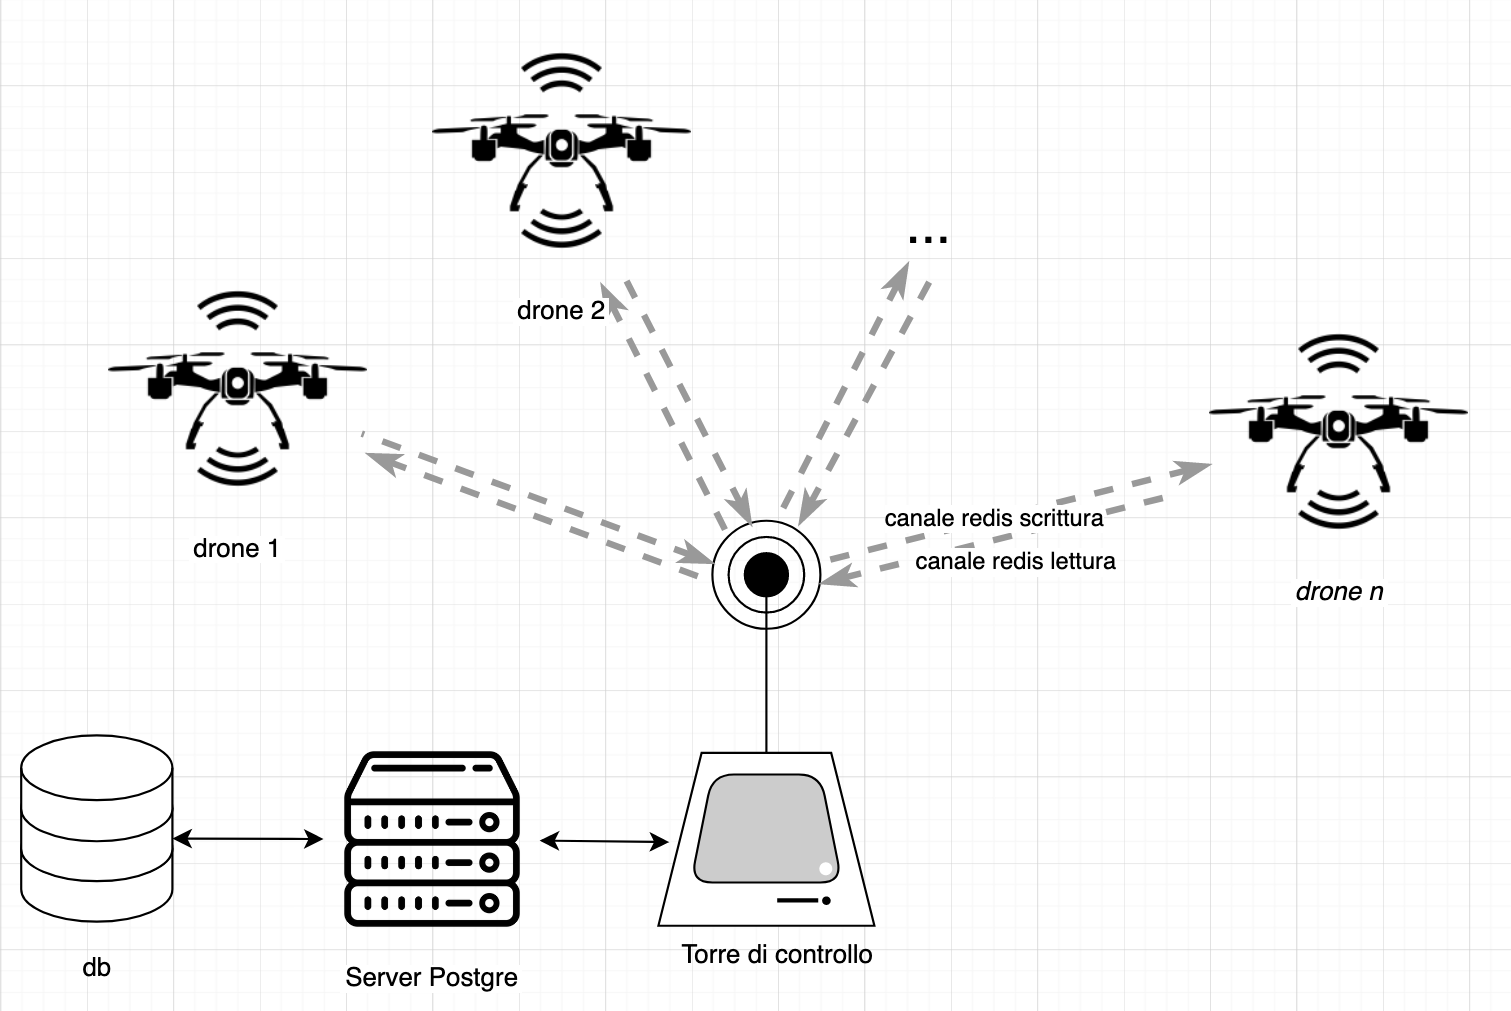
\includegraphics[height = 7.2 cm]{image/Architettura.png}\\
    \caption{Architettura fisica del sistema}
\end{figure}
\newpage

\section{Analisi del software}
\subsection{Requisiti utente}
Per funzionare, il sistema ha bisogno dei seguenti requisiti:
\begin{itemize}
    \item dimensione dell'area\\
    dato che l'area verrà divisa in blocchi, per ogni blocco è di interesse:
    \begin{itemize}
        \item limite alto superiore
        \item limite basso inferiore
        \item punto di partenza (o ultimo punto visitato)
        \item Ogni punto dell'area è identificato dalla sua posizione in una matrice di punti e di quei punti ci interessa solo:
        \begin{itemize}
            \item il tempo trascorso dall'ultima visita.
        \end{itemize}
    \end{itemize}
    \item numero di droni\\
    per ogni drone è di interesse:
    \begin{itemize}
        \item id: identificativo univoco seriale
        \item Stato : tra i stati precedentemente elencati
        \item posizione 
        \item carica residua (in minuti)
        \item carica massima (in minuti)
        \item tempo di ricarica 
        \item last\_update : tempo trascorso dall'ultimo update
    \end{itemize}
    
\end{itemize}
\newpage
\subsection{Requisiti di sistema}
Il sistema deve rispettare i seguenti requisiti:
\begin{enumerate}
    \item Area:
    \begin{enumerate}[label=1.\arabic*]
        \item I blocchi sono tutti tra loro disgiunti (non esiste un punto dell'area che si trova in più di un blocco)
        \item L'unione dei blocchi copre tutti e solo i punti dell'area (un punto appartiene all'area se e solo se esiste un blocco che lo contiene)
        \item Un blocco può essere assegnato al più ad un drone 
    \end{enumerate}
    \item Drone:
    \begin{enumerate}[label=1.\arabic*]
        \item Un drone a cui è stato assegnato un blocco può trovarsi al di fuori di esso se e solo se:
        \begin{enumerate}
            \item il drone è partito dalla torre e si sta posizionando verso il punto di partenza del blocco
            \item il drone è scarico e sta tornando alla torre
            \item il drone ha visitato tutto il blocco e si sta posizionando verso il punto di partenza di un'altro blocco
        \end{enumerate}
        \item Un drone può volare verso un punto diverso da quello della torre se e solo se il suo tempo di volo residuo è maggiore del tempo che serve al drone per andare dalla sua posizione attuale a quella della torre
    \end{enumerate}
    \item Torre:
    \begin{enumerate}[label=1.\arabic*]
        \item La torre non può terminare il suo processo se esiste un drone connesso che non è tornato nella torre di controllo.
        \item Tutti i punti che la torre invia ad un drone devono trovarsi all'interno dell'area assegnata al drone
    \end{enumerate}
    \item Requisiti non-funzionali:
    \begin{enumerate}[label=1.\arabic*]
        \item ogni punto dell'area deve essere visitato il più frequentemente possibile
        \item Il tempo di risposta della torre per ogni drone deve essere ragionevolmente basso per fare in modo che i droni rimangano fermi sul posto il meno possibile
    \end{enumerate} 
\end{enumerate}
\newpage
\subsection{Diagrams}
\begin{figure}[htbp]
    \centering
    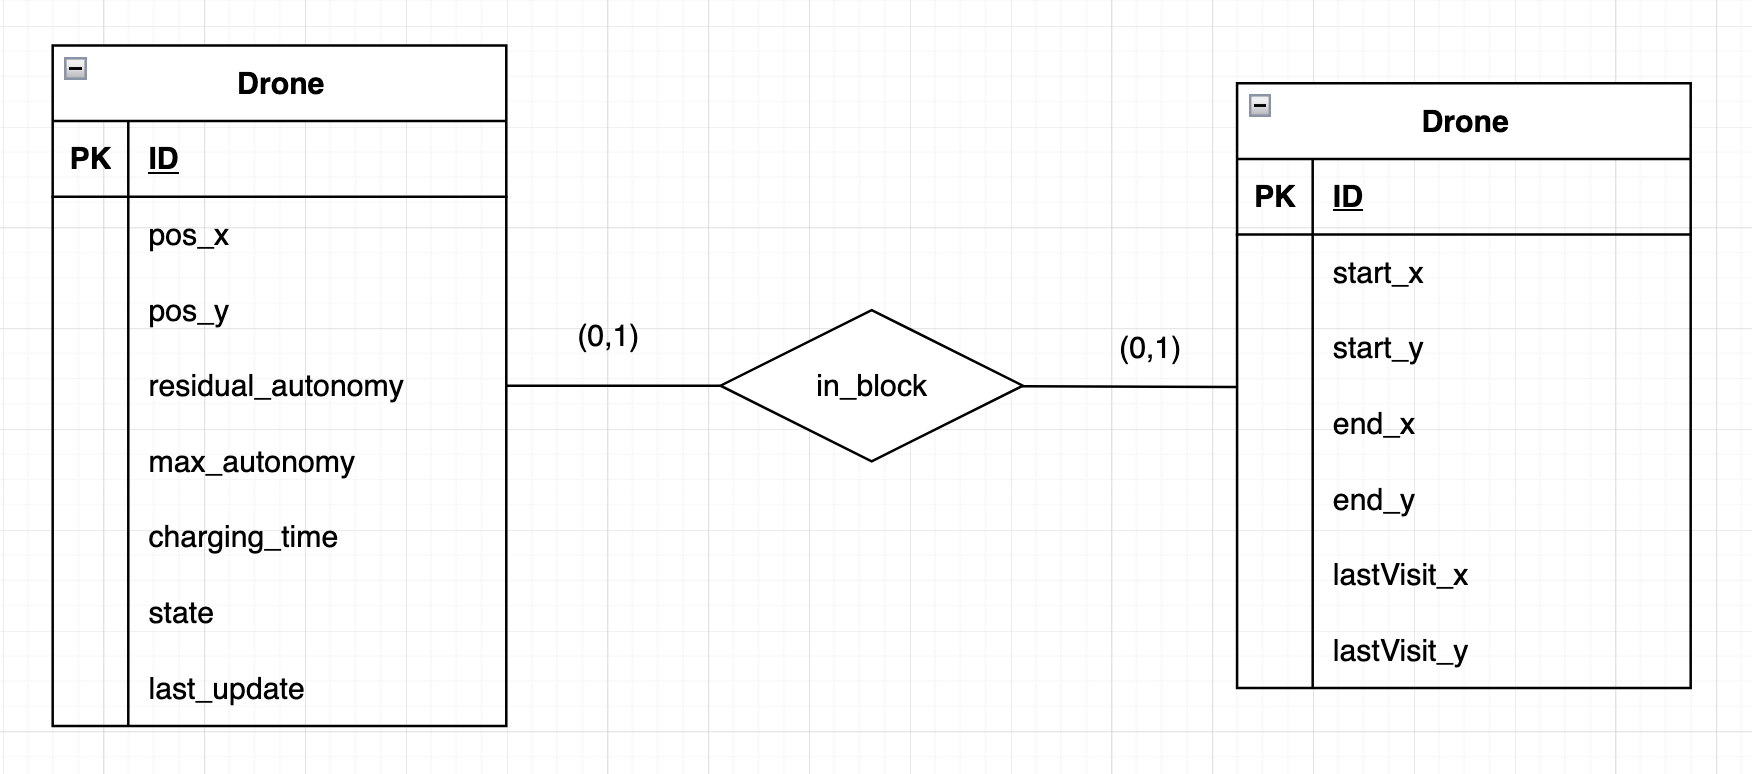
\includegraphics[height = 4 cm]{image/ER1.png}%
    \qquad\qquad
    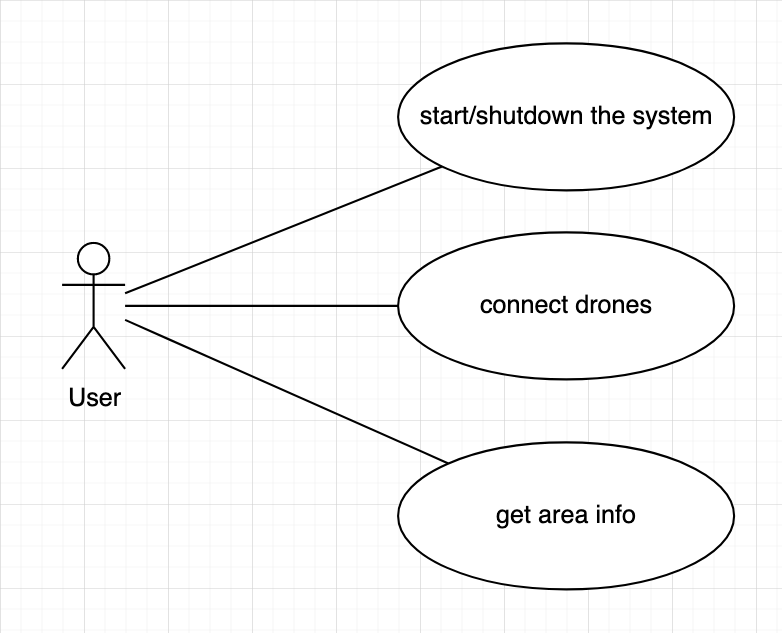
\includegraphics[height = 4 cm]{image/UML1.png}
    \caption{schema ER e UML}
\end{figure}


\subsection{Algoritmo}
Contando di poter ottenere per ogni drone, una tupla contenente almeno \{\textit{Id, Posizione, Stato, Blocco}\} di tutti i droni che si sono connessi alla torre e le dimensioni dell'area da sorvegliare, la torre inizia a seguire il seguente algoritmo.
Il problema può essere gestito seguendo i seguenti passaggi:
\begin{enumerate}
    
    \item La torre di controllo conta i droni che si sono connessi e divide l'area da sorvegliare in $N$ blocchi \underline{tutti della stessa misura}
     secondo una specifica funzione che fa in modo di avere più blocchi che droni.

    \item La torre assegna ad ogni drone \textit{"pronto a partire"} un blocco disponibile.

    \item Ogni drone si dirige al punto di partenza del blocco assegnatogli. Non appena lo raggiunge lo comunica alla torre.

    \item Quindi la torre azzera il tempo di visita dell'area $20\times 20$ centrata nella posizione del drone e gli invia il prossimo punto da raggiungere
     per scansionare tutto il blocco.

    \item Quando il drone ha visitato tutto il blocco gli viene assegnato il blocco disponibile che contiene il punto non visitato da più tempo. Il loop continua dal punto 3.
    \item Quando un drone ha carica appena sufficiente per tornare alla torre di controllo parte la procedura di return. 
    Segnala alla torre che sta tornando comunica quindi l'ultimo punto visitato e si dirige alla torre.
    
    \item Quando il drone arriva alla torre di controllo inizia a ricaricarsi.
    La torre lo marchera come \textit{"pronto a partire"} non appena la batteria sarà carica.

    \item Se la torre non riceve messaggi da un drone in volo per troppo tempo questo verrà segnato come \textit{"morto"}. 
\end{enumerate}
Questo è l'idea principale per far si che tutti i punti vengano visitati il più frequentemente possibile.
Questo ciclo viene ripetuto finche l'utente non interrompe il programma o tutti i droni "muoiono".
\begin{figure}[h]
    \centering
    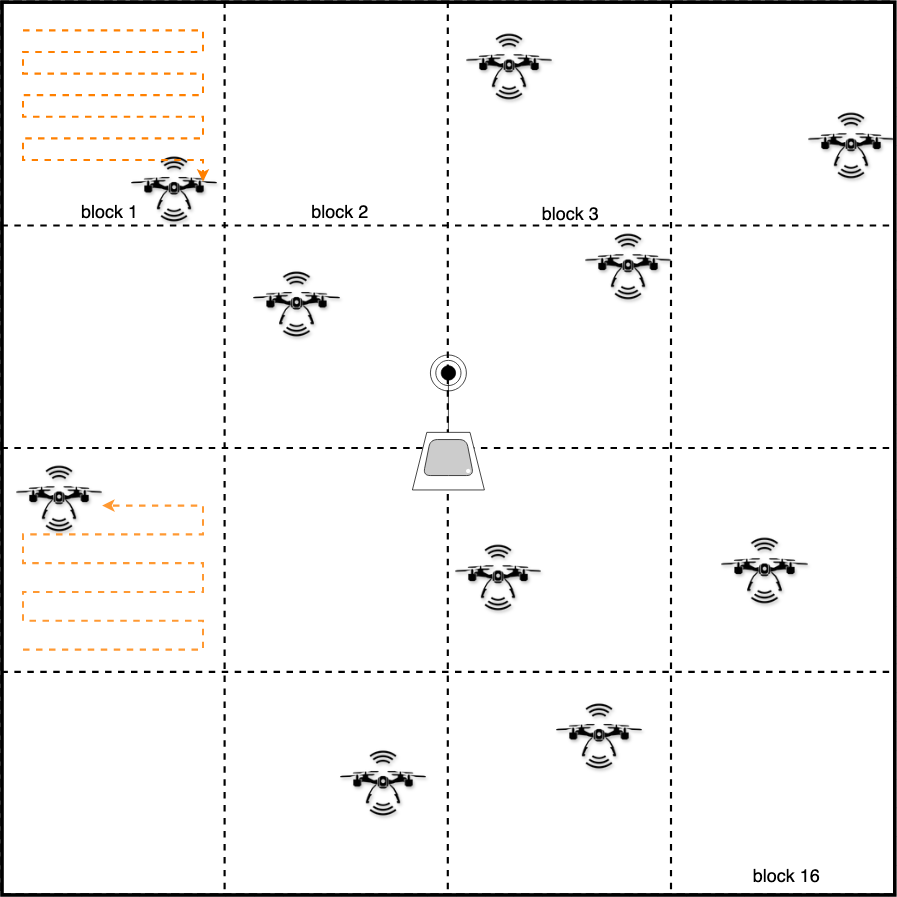
\includegraphics[height = 8 cm]{image/DroniInArea.png}%
    \ 
    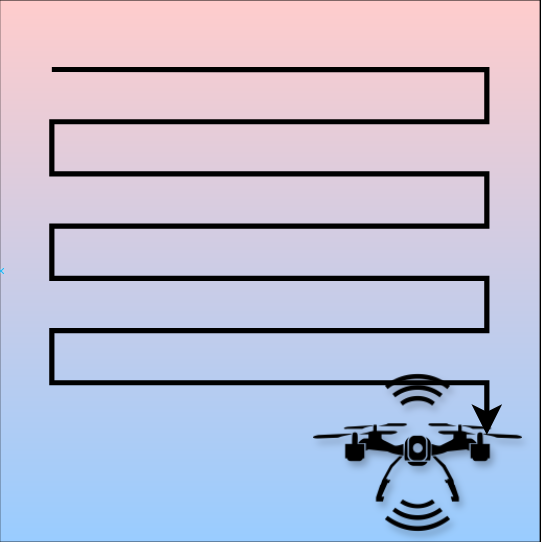
\includegraphics[height = 4 cm]{image/DroneInBlock.png}
    \caption{Esempio di area suddivisa in blocchi. Nel dettaglio a destra oltre al percorso seguito dal drone, viene evidenziata come più "calda" l'area visitata da meno tempo e più "fredda" l'area appena vista.}
\end{figure}

\begin{figure}[H]
    \centering
    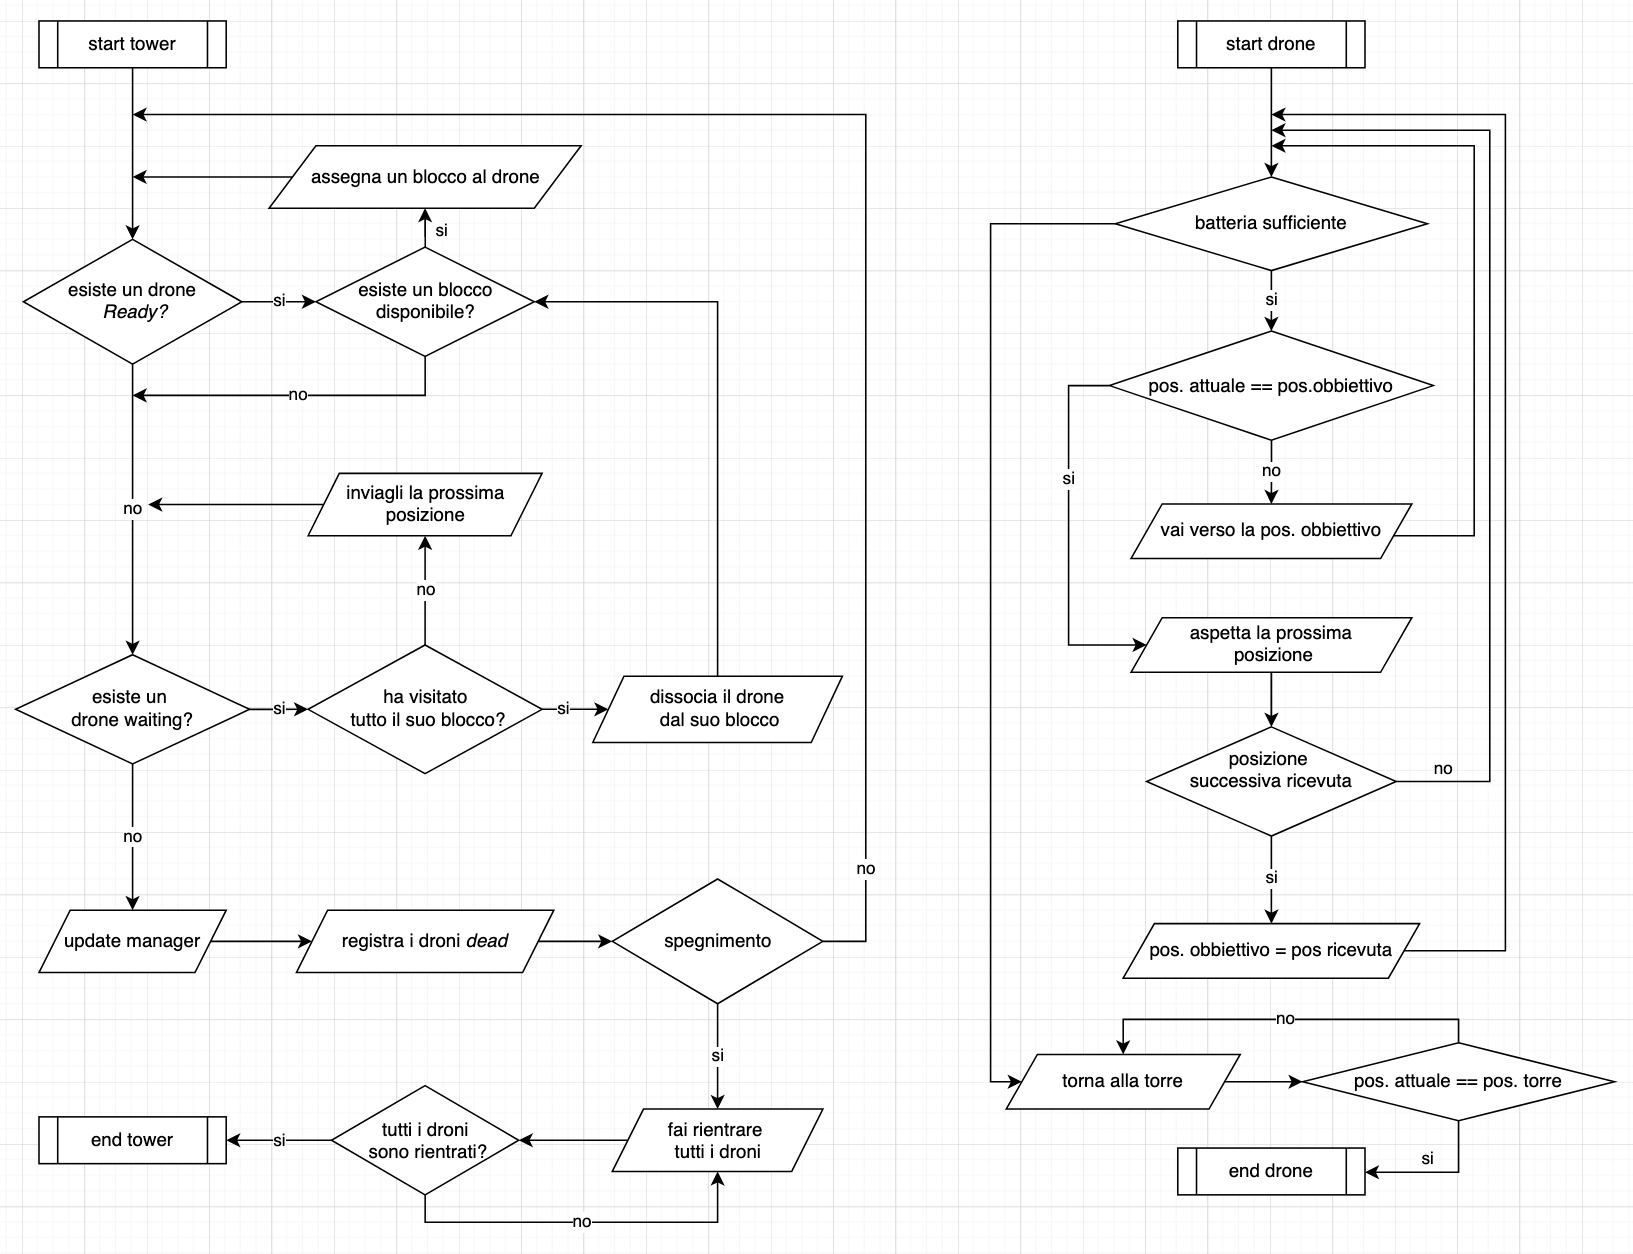
\includegraphics[height = 16 cm]{image/FlowCharts.png}
    \caption{FlowChart della torre e del drone. Nota bene, nel FlowChart viene assunto che il drone e la torre siano già connessi}
    
\end{figure}

\begin{figure}[H]
    \centering
    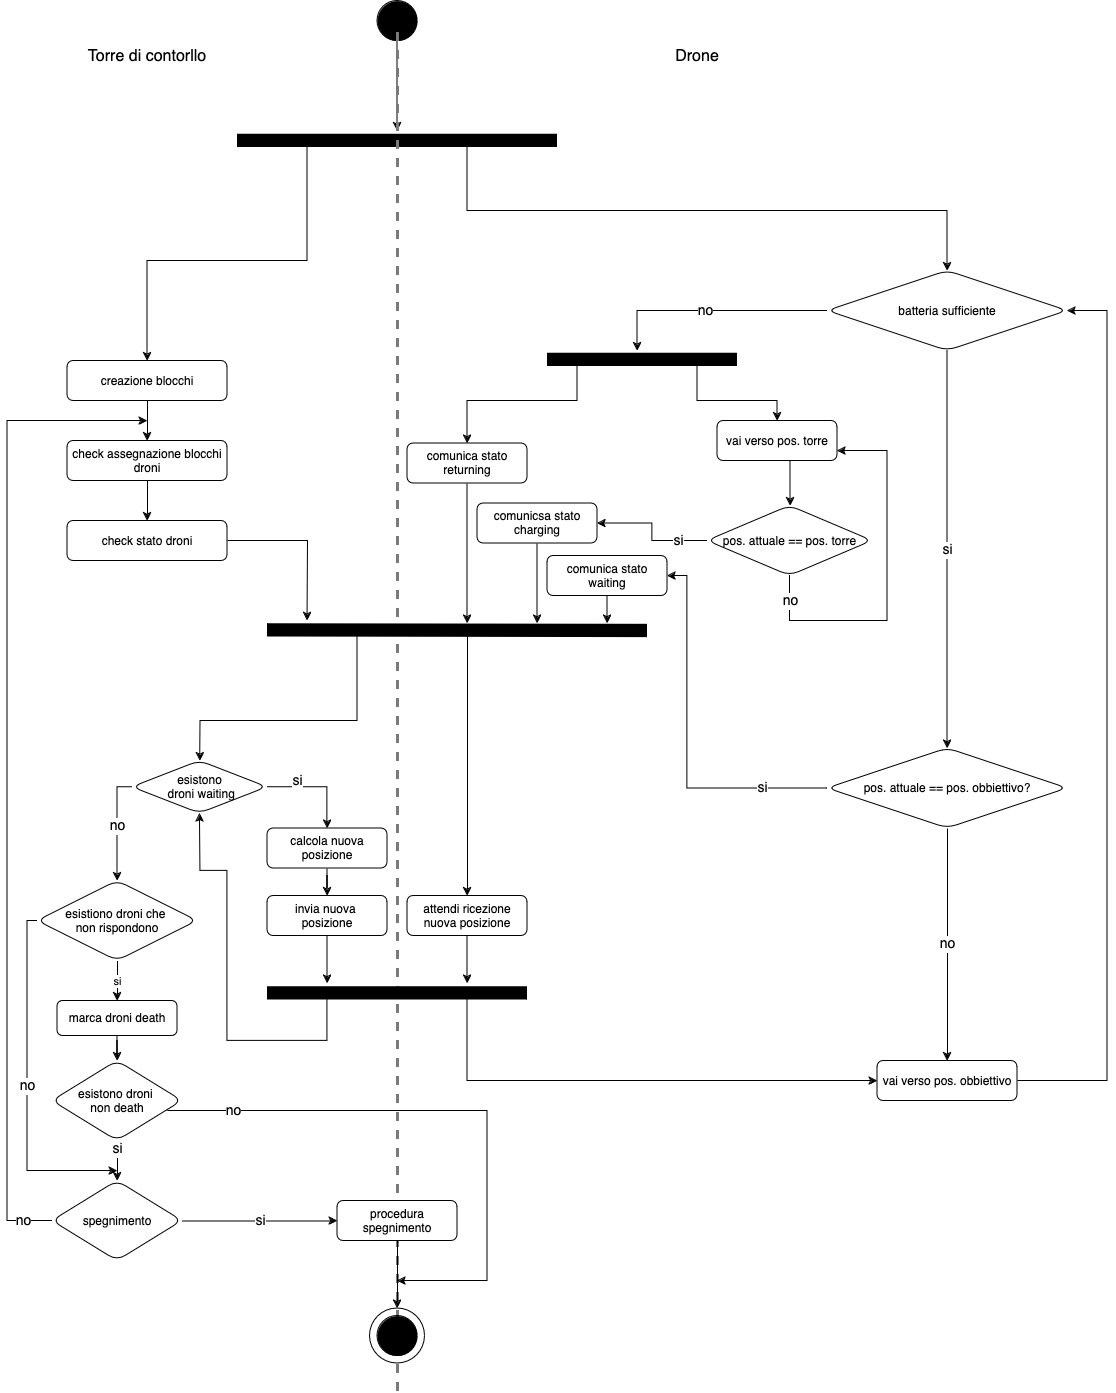
\includegraphics[height = 17 cm]{image/activitiDiagram.png}
    \caption{Activity diagram del sistema di interazione e decisione tra torre e drone, nel diagramma sono mostrate due barriere in cui drone e torre si sincronizzano per scambiarsi i messaggi principali mentre è lasciato implicito l'handler message di entrambi per messaggi di check.}
    
\end{figure}


\newpage
\subsubsection{State diagram}
Per decidere l'azione da assegnare ad ogni drone la torre deve riuscire a distinguere la condizione di ogni drone. 
Definiamo quindi $6$ stati in cui ogni drone può trovarsi:
\begin{enumerate}
    \item \textbf{CHARGING:} il drone si trova alla base, e sta ricaricando la sua batteria
    \item \textbf{READY:} il drone è carico e si trova nella torre di controllo (è pronto a partire)
    \item \textbf{WAITING:} il drone sta aspettando che la torre gli invii la prossima coordinata
    \item \textbf{MONITORING:} il drone sta scansionando l'area che gli è stata assegnata seguendo i punti inviati dalla torre
    \item \textbf{RETURNING:} la carica del drone è sufficiente solo per il suo rientro (il drone sta rientrando)
    \item \textbf{DEAD:} la batteria del drone si è scaricata prima che questo potesse rientrare oppure la torre di controllo non riesce più a contattarlo (fault).
\end{enumerate}
\begin{figure}[h]
    \centering
    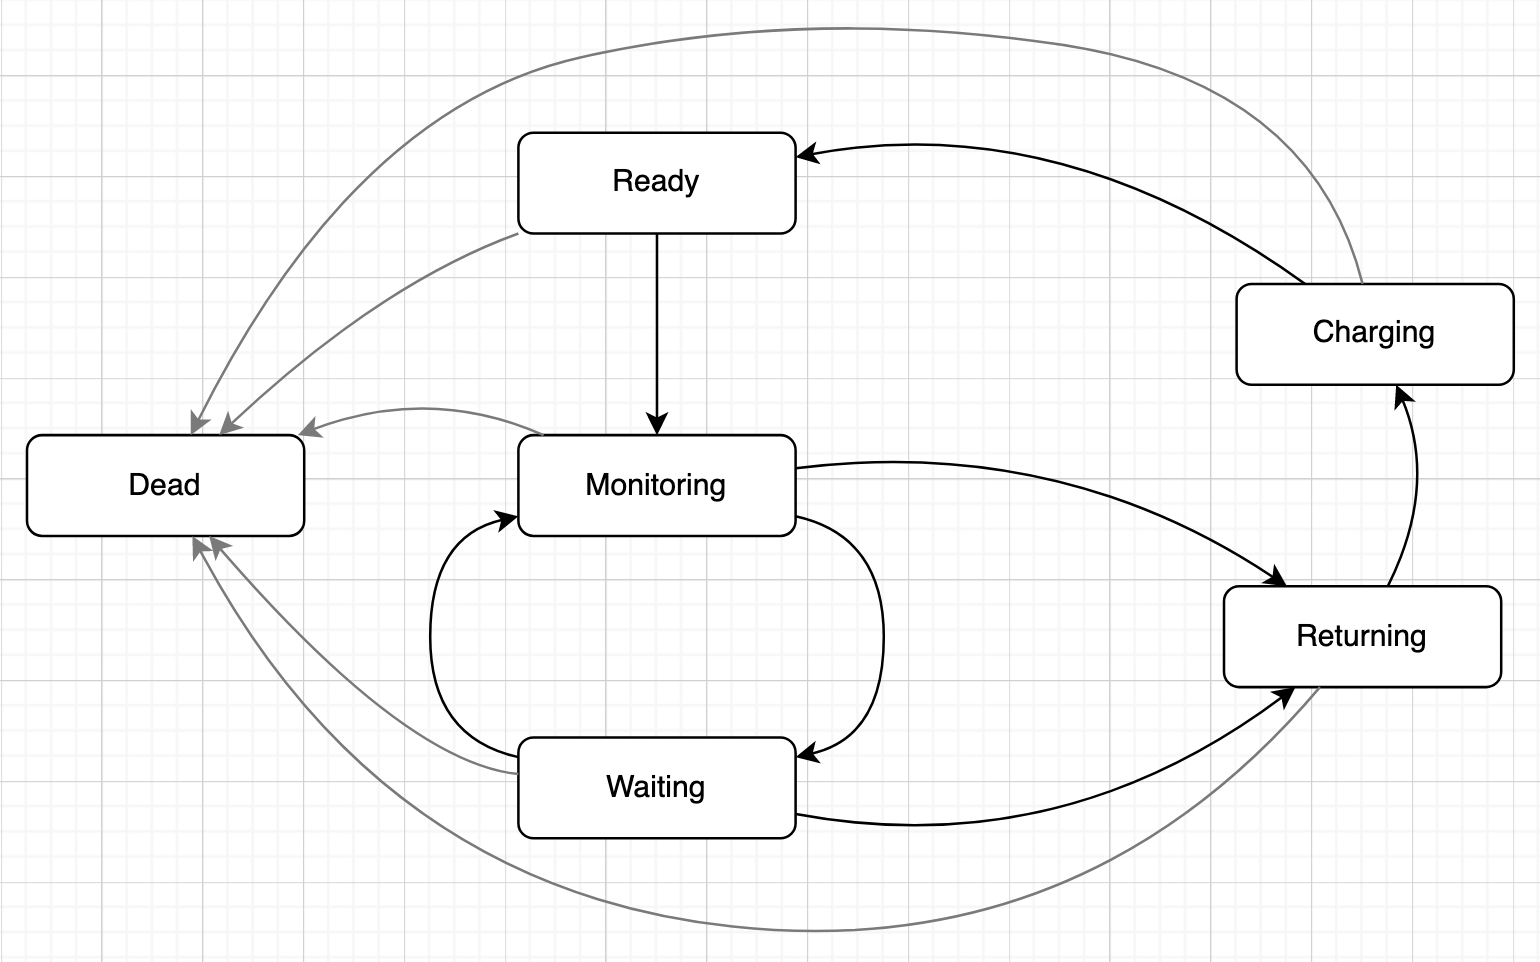
\includegraphics[height = 8 cm]{image/StateDiagram.png}
    \caption{State diagram}
\end{figure}
\subsubsection{Scelte progettuali}
\paragraph*{Divisione dei blocchi}
Dato che un punto si considera visitato se si trova nel raggio di 10 metri da un drone, possiamo discretizzare l'area rappresentandola come una matrice di case quadrate di dimensione $10\sqrt(2) \times 10\sqrt(2)$
\begin{figure}[h]
    \centering
    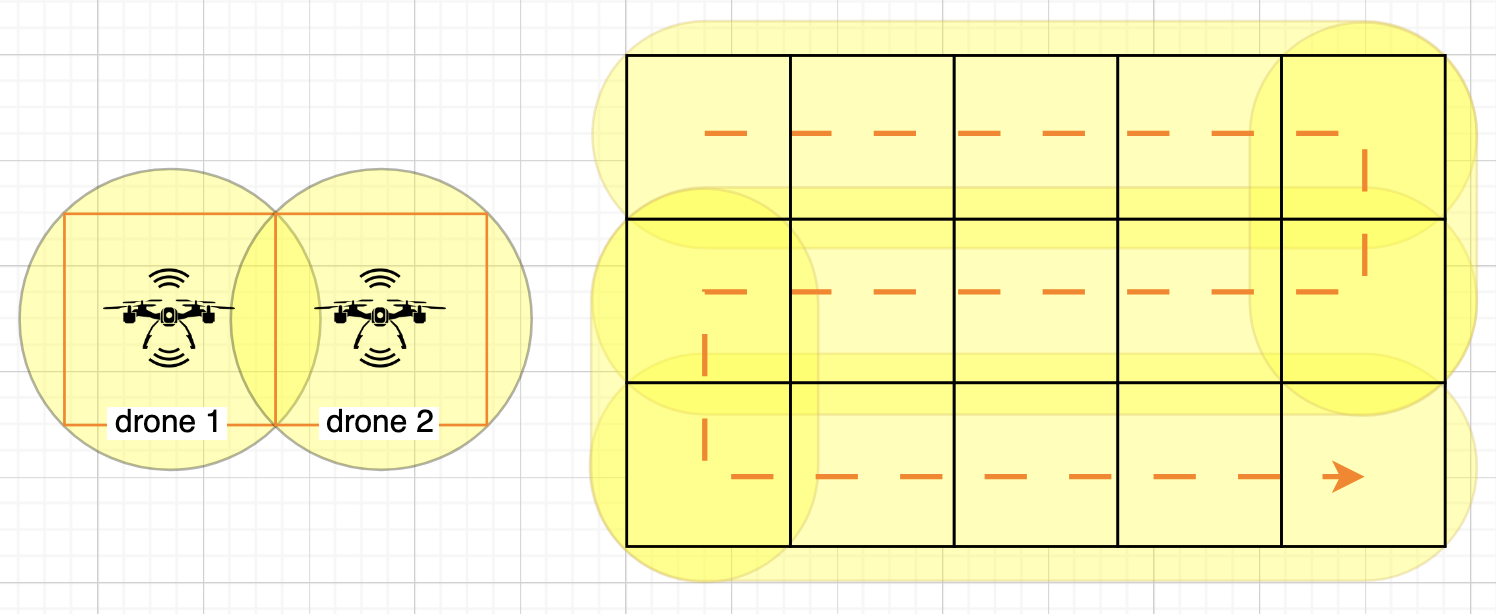
\includegraphics[height = 5 cm]{image/areedroni.png}
    \caption{L'area divisa in caselle della dimensione del quadrato inscritto nel cerchio di raggio 10}
\end{figure}

Abbiamo scelto di raggruppare le caselle in blocchi tutti uguale area per garantire equità nelle assegnazioni. 
Data la variabilità delle dimensioni dell'area e del numero di droni in fase iniziale, non è sempre garantito che il numero di droni divida il numero caselle in un valore utile per costruire una matrice di blocchi, utilizziamo un valore di blocchi maggiore per garantirne la perfetta di visibilità in sottoaree uguali.
Questo permette a tutti i droni \textit{READY} di volare contemporaneamente all'inizio del processo di monitoraggio e quindi ridurre il più possibile il tempo di visita medio dell'intera area.
Anche se creare più blocchi ne riduce le dimensioni, questo non influisce sulle prestazioni del sistema in quanto ogni drone quando termina il ciclo di visita del suo blocco inizia a visitarne un altro e continua finché la batteria lo permette.


\paragraph*{Assegnamento dei blocchi}
Per minimizzare il tempo di visita massimo e medio abbiamo sperimentato due criteri di scelta:
\begin{enumerate}
    \item \textbf{FirstAverageTime}: Assegnare ad un drone \textit{free} il blocco con tempo medio trascorso dall'ultima visita più alto (la media viene eseguita su tutte le caselle nel blocco).
    
    \item \textbf{FirstMaxTime}: Assegnare ad un drone \textit{free} il blocco che contiene la casella visitata meno di recente.
\end{enumerate}
Attualmente il programma utilizza il secondo approccio (\textbf{FirstMaxTime}). Se valutiamo il criterio di assegnamento basandoci su tempo di visita medio e tempo di visita massimo raggiunto durante una simulazione, 
possiamo osservare che a parità di area e di droni il FirstAverageTime ottiene un tempo di visita medio leggermente più basso di quello del FirstMaxTime ma un tempo massimo più alto in quanto tende a non riassegnare dei blocchi (magari quelli più ai margini) che hanno pochi punti con un tempo di visita molto alto ma molti con tempo di visita molto basso.
Al contrario il FirstMaxTime al costo di aumentare leggermente il tempo medio di visita, riesce a diminuire sensibilmente il tempo di visita massimo dimostrandosi più equo.  



\end{document}